\documentclass{paper}
\usepackage{times}
\usepackage{geometry}
\geometry{letterpaper, portrait, margin=1in}
\usepackage[utf8]{inputenc}
\usepackage{enumitem,amssymb}
\usepackage{ragged2e}
\usepackage{physics}
\usepackage{siunitx}
\usepackage{float}

\usepackage{caption}
\usepackage[hidelinks]{hyperref}
\usepackage{url}

\usepackage{graphicx}
\usepackage{epstopdf}
\graphicspath{{data/cos-w5}}

\usepackage{biblatex}
\bibliography{refs}

\title{cos-w5 tasks}
\author{ariahayd}
\date{1 March 2022}

\begin{document} 

\maketitle

\begin{enumerate}
    \item % 1.
      Mattig's Formula is defined in Eq. \ref{eqn:mattig}

      \begin{equation}
        r R_0 = \frac{2c}{H_0}\left[ \frac{\Omega_0 z + 
        ( \Omega_0 -2 )[(1+\Omega_0 z)^\frac{1}{2} - 1]}
        {\Omega_0^2 (1+z)}\right]
        \label{eqn:mattig}
      \end{equation}

      A simplification for the Einstein-de-Sitter cosmology, a flat,
      matter-dominated universe, implies \(\Omega_0 = 1\):

      \[ r R_0 = \frac{2c}{H_0}\left[\frac{z+(1-2)[(1+z)^\frac{1}{2}-1]}
        {(1+z)}\right]
        = \frac{2c}{H_0}\left[ \frac{(1+z)-(1+z)^\frac{1}{2}}{(1+z)}\right]
        = \frac{2c}{H_0}\left[ 1-(1+z)^\frac{1}{2}\right]
      \]

      Find the maximum \(d_A\) value between \(1<z<2\) for the angular
      diameter distance in Eq. \ref{eqn:da}

      \begin{equation}
        d_A = \frac{2c}{H_0(1+z)}\left[1-(1+z)^{-\frac{1}{2}}\right]
        \label{eqn:da}
      \end{equation}

      Eq. \ref{eqn:da} can be rewritten to be more easily differentiated as:
      \[
        d_A = \frac{2c}{H_0}\left[z-(1+z)^\frac{1}{2} +1\right]
      \]

      Differentiate to find the inflection point:
      \[
        \frac{\dd{(d_A)}}{\dd{z}} = \frac{2c}{H_0} - 
        \frac{\dd{}}{\dd{z}}\left[\frac{2c}{H_0}(1+z)^\frac{1}{2}\right]
        = \frac{2c}{H_0}\left[1-\frac{1}{2}(1+z)^{-\frac{1}{2}}\right]
      \]

      Solve for where differential is zero:
      \[
        1-\frac{1}{2}(1+z)^{-\frac{1}{2}} = 0
        \implies (1+z)^{-\frac{1}{2}} = 2 \implies z = 1 + \frac{1}{4}
      \]

      Given the maxiumum size of the distance \(s\) between two points that
      may be causally connected at decoupling, \(s=ct_d\). Use Eq.
      \ref{eqn:da} to estimate the angular size, \(\theta\) where
      \(\tan{\theta} = \frac{s}{d_A} \implies \theta \approx \frac{s}{d_A}\)
      for small angles of \(\theta\).

      \[
        \theta \approx \frac{s}{d_A} = \frac{ct_d}
        {\frac{2c}{H_0}\left[(1+z)-(1+z)^\frac{1}{2}\right]}
      \]

      Substitute \(\frac{1}{H_0}\) as the Hubble time, \(t_H\), with
      \(z = 1000\), \(t_d = 3.8e^5 \si{years}\), and 
      \(t_H = 14.4e^9 \si{years}\),
      \[
        \theta \approx \frac{t_d}{2t_H}\left(\frac{1}{1001-\sqrt{1001}}\right)
        = 1.36e^{-8} \si{radians} = 7.79e^{-7} \si{degrees}
      \]

    \item % 2.
      The redshift resulting in a maximum angular diameter distance,
      \(d_A\), with sensible parameters \(\Omega_{m,0} = 0.3\) and
      \(\Omega_{\Lambda,0} = 0.7\) is shown in Fig. 
      \ref{fig:angular-diameter-distance}. This chart indicates a maximum
      value of approximately \(z = 1.5\).
      \begin{figure}[H]
        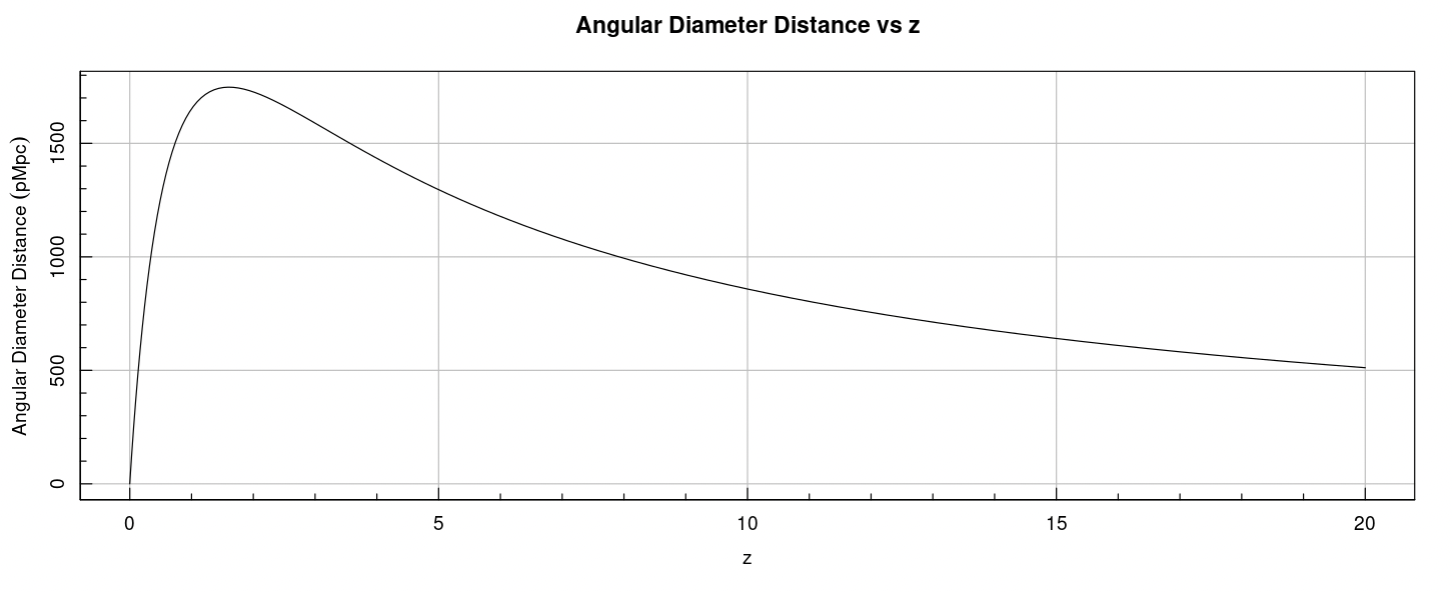
\includegraphics[width=\linewidth]{angular-diameter-distance.png}
        \caption{Calculated angular diameter distance by redshift, shown
        in decreasing horizontal axis}
        \label{fig:angular-diameter-distance}
      \end{figure}

      Figs. \ref{fig:omega-m}, \ref{fig:omega-l}, and \ref{fig:omega-r} 
      are plots of each density parameter \(\Omega\) as a function of 
      \((1+z)\) over the domain of \(z < 1600\).

      \begin{figure}[H]
        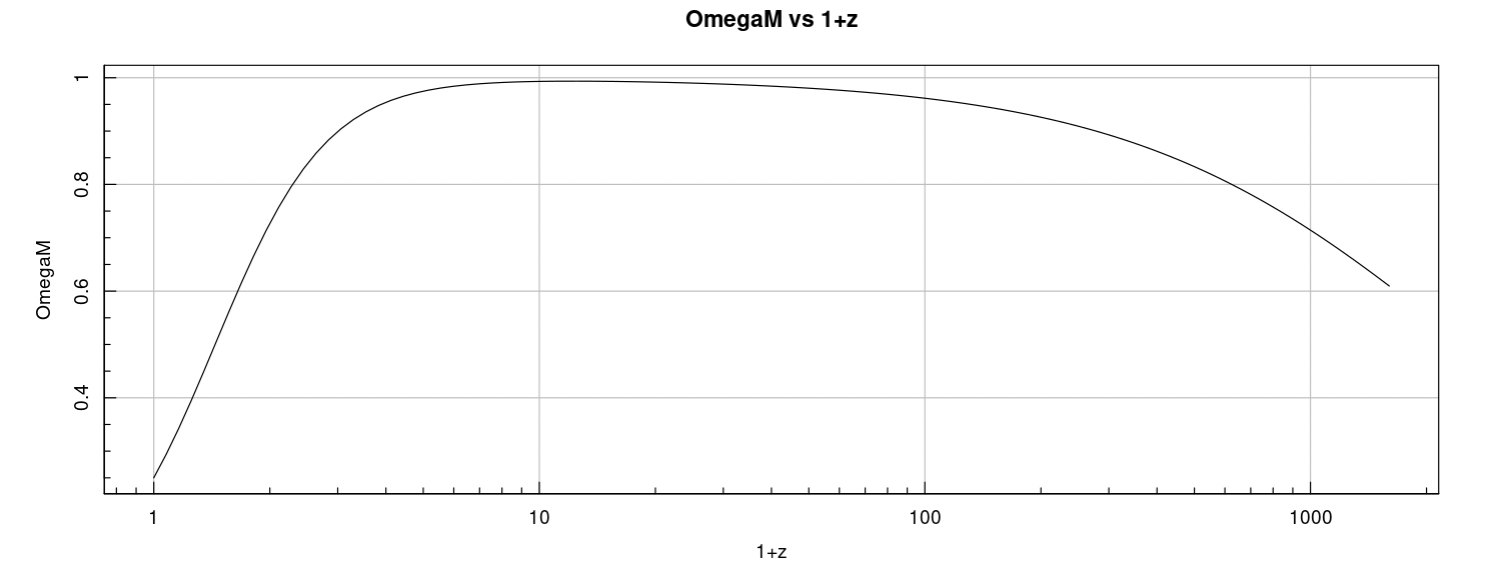
\includegraphics[width=\linewidth]{omega-m.png}
        \caption{Density parameter for matter per \((1+z)\)}
        \label{fig:omega-m}
      \end{figure}

      \begin{figure}[H]
        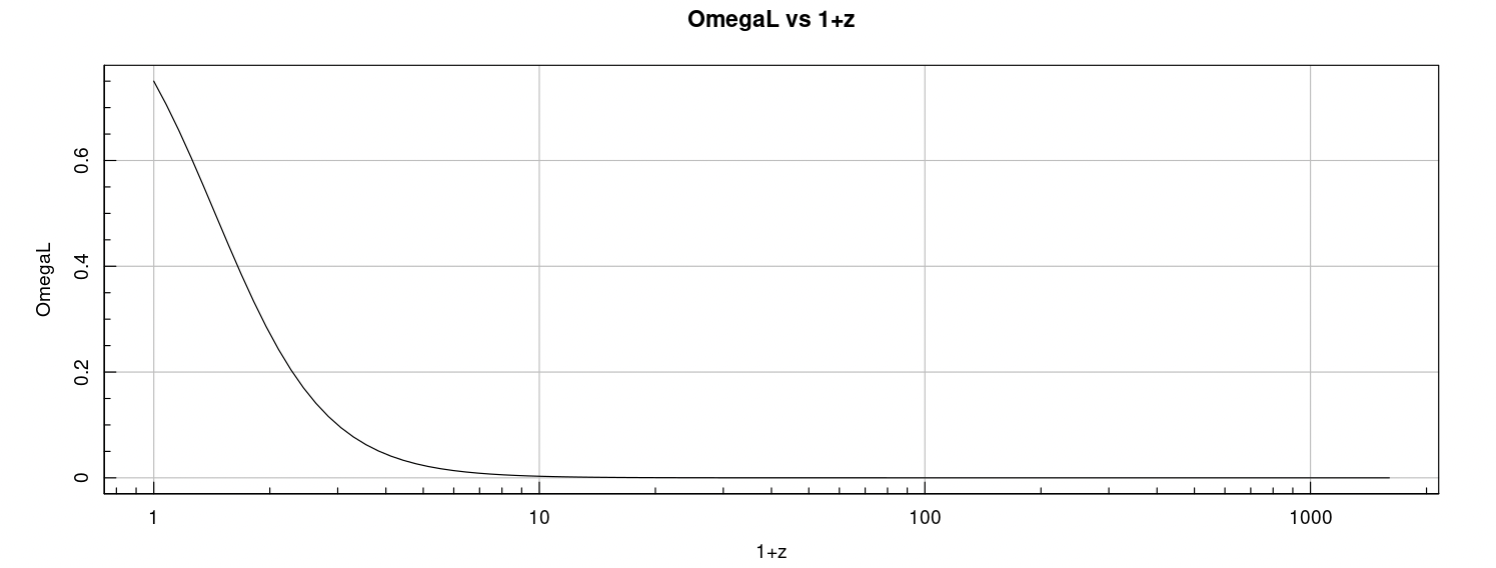
\includegraphics[width=\linewidth]{omega-l.png}
        \caption{Density parameter for expansion energy per \((1+z)\)}
        \label{fig:omega-l}
      \end{figure}

      \begin{figure}[H]
        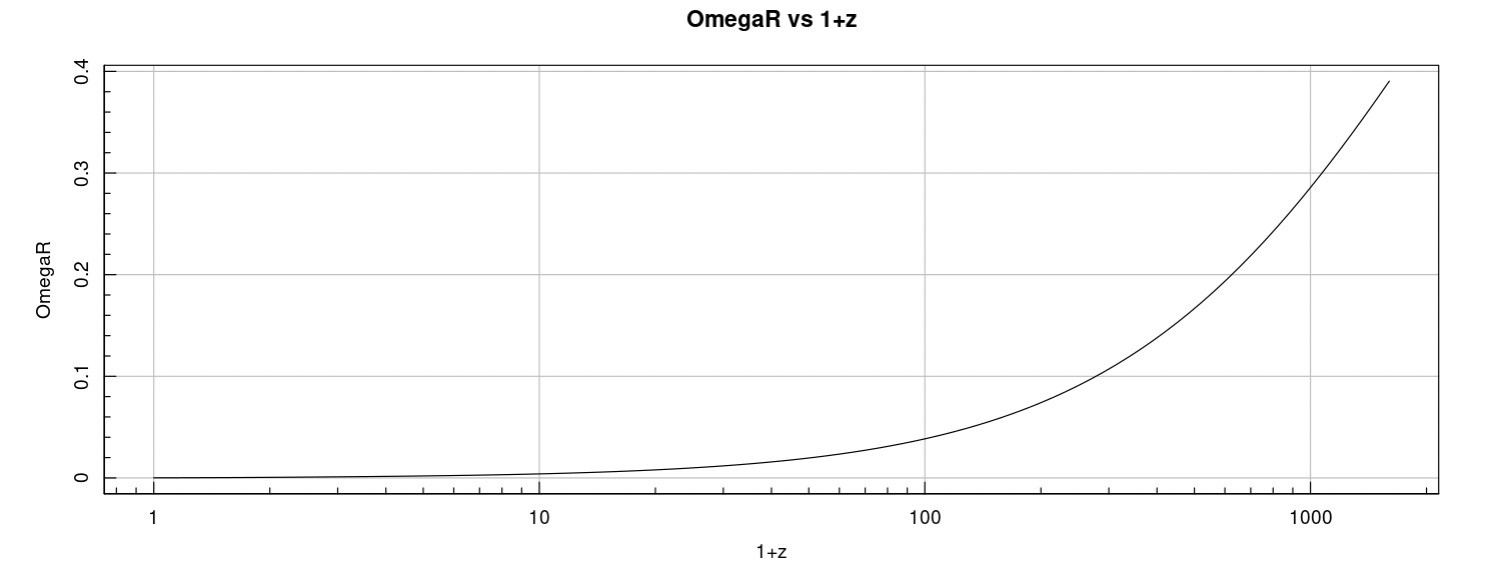
\includegraphics[width=\linewidth]{omega-r.png}
        \caption{Density parameter for radiation per \((1+z)\)}
        \label{fig:omega-r}
      \end{figure}

      The radiation-dominated era of the universe, when the density
      parameter due to radiation alone was large, \(\Omega_r > 0.9\),
      occured at approximately \(10e^{-6} \si{Gyr}\), as shown by Fig.
      \ref{fig:radiation-age}.

      \begin{figure}[H]
        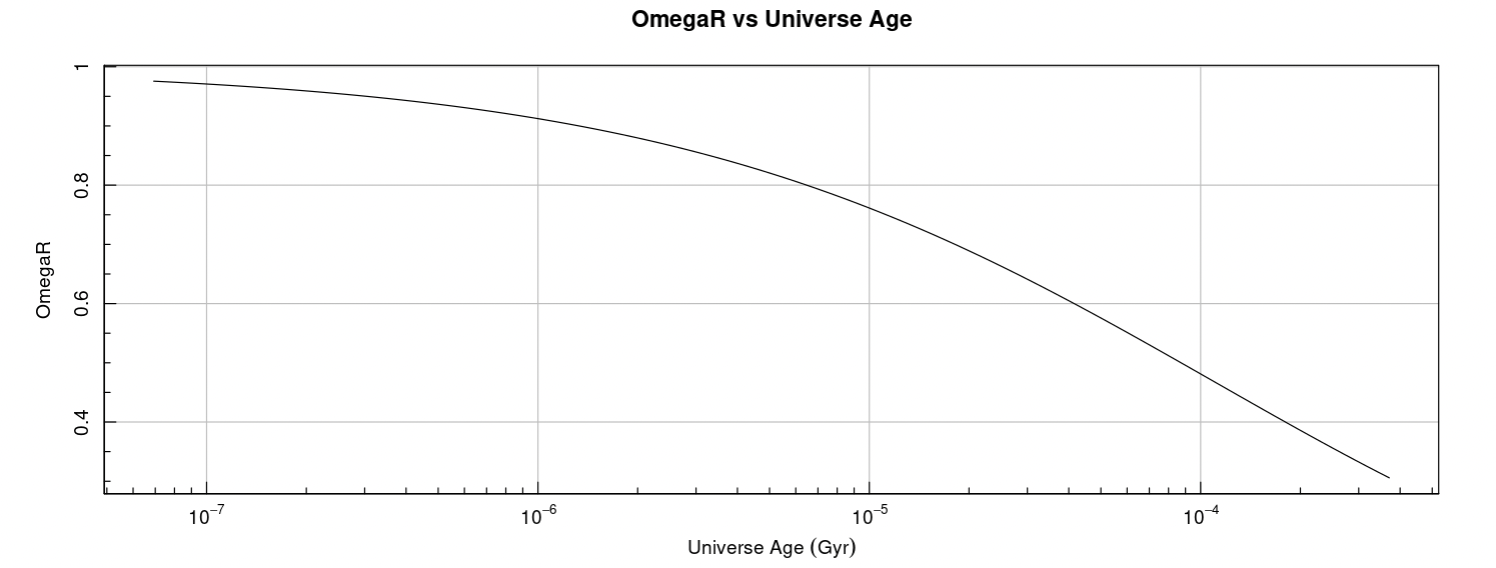
\includegraphics[width=\linewidth]{radiation-age.png}
        \caption{Plot of radiation dominance per universe age}
        \label{fig:radiation-age}
      \end{figure}

    \item % 3.
      Einstein knew that a spacetime curved by gravitation is not a stable
      system on long times scales. Either the system collapses on itself due
      to self gravitation from an energy density greater than the critical
      density or it expands infinitely with masses moving apart forever.
      Neither longtime scenario matched observations at the time, which
      predicted a steady state. He embedded a term \(\Lambda\) to force the
      steady state by balancing mass density of self-gravitation with a 
      negative energy density.

      For the cases of \(\Omega_{\Lambda}=0\), \(\Omega_m=1\), explain the
      differences versus the current \textit{737} model with 
      \(\Omega_{\Lambda}=0.7\), \(\Omega_m=0.3\):

      \begin{enumerate}
        \item % a.
          In the \textit{737} model, \(\Omega_\Lambda\) is significant to
          redshifts \(< 10\). In the matter-dominated model with 
          \(\Omega_\Lambda = 0\), there is no contribution from cosmological
          expansion. Between the two models, there is no difference in 
          expansion in the early universe.

        \item % a.
          The flat, matter dominated model underestimates the overall age of
          the universe. \(\Omega_m = 1\) results in a lookback time of 
          \(\frac{2}{3}\) the current Hubble time, which is less than the
          measured age of some stellar clusters. With the \textit{737}
          model, the age of the universe is measured to be the Hubble time.

        \item % a.
          Both models are based on the total density parameter equal to
          unity, \(\Omega = 1\), resulting in a flat geometry and neverending
          expansion of space. However, in the \textit{737} model, expansion
          accelerates over time once \(\Omega_\Lambda > 0.15\) of the sum
          of density parameters.

      \end{enumerate}

    \item % 4.
      The acceleration parameter, \(q\), reflects any dominance of the
      expansion density parameter, \(\Omega_\Lambda\) over the 
      self-gravitation density parameter, \(\Omega_m\). Negative values
      of \(q\) imply accelerating expansion.

      Where \(q=0\) is the inflection point that balances acceleration
      in expansion and contraction.

      \[
        q = 0 = \frac{\Omega_m}{2}-\Omega_\Lambda \implies
        \Omega_\Lambda \geq \frac{1}{2}\Omega_m 
      \]

      For the observed value of \(\Omega_m = 0.3\), any value of 
      \(\Omega_\Lambda > 0.15\) will cause accelerating expansion.

    \item % 5.
      A \textit{geometric} method for measuring cosmic distances is to 
      observe a distant source at different points in the orbit of Earth
      around the Sun to measure the parallax of the source against the
      background of objects more distant than it. Parallax can be measured
      for sources \(< 5 \si{kpc}\).

      One \textit{standard candle} method for measuring distance is to 
      measure the timing in the decline of the lightcurve from a type 1a
      supernova. The duration of the curve can be fit to a stellar model
      to determine the intrinsic luminosity of the star. These events are
      bright enough to see in distant galaxies, but are rare.
      
    \item % 6.
      What is the greatest error allowable in the mesaurement of parallax
      of a point source at a distance of \(5 \si{kpc}\) from a near-Earth
      orbital telescope that allows less than 10\% error in the distance
      measurement?
      \[
        d(\si{pc}) = \frac{1 \si{AU}}{p"} \implies
        \Delta d(\si{pc}) = \frac{1 \si{AU}}{\Delta p\si{''}}
      \]

      Where \(\Delta d = 10\% \times 5 \si{kpc}\),
      \[ 
        \Delta p(\si{''}) = \frac{1 \si{AU}}{10\% \times 5 \si{kpc}} 
        = 9.70e^{-9} \si{radians} = 0.002 \si{arcsec}
      \]

    \item % 7.
      Measurements of photon sources at signficant redshifts are challenged
      by the following:

      \begin{enumerate}

        \item
          Scientific instruments are moving with respect to the rest frames
          of the sources being observed. This relative motion must be
          compensated for.

        \item
          Measure distances using galaxies as in indicators requires 
          correcting the expected light profile from the galaxy as it is 
          shifted from the source rest frame and due to the evolution
          effects in the stellar populations within the galaxy.

        \item
          Dust in the ecliptic plane of the Milky Way cause extinction of 
          source where the light must travel through the plane.

        \item
          Sources at high redshift are dimmed as \((1+z)^2\). This extra 
          dimming makes it more difficult to measure the dim objects within
          a distant region of space than within a nearby region of space,
          causing selection effects.

      \end{enumerate}


\end{enumerate}

This paper is available publicly.\cite{Hayden_Cosmology_Source_Repo}

\pagebreak
\printbibliography

\end{document}

